% book example for classicthesis.sty
\documentclass[
  % Replace twoside with oneside if you are printing your thesis on a single side
  % of the paper, or for viewing on screen.
  %oneside,
  oneside,
  11pt, a4paper,
  footinclude=true,
  headinclude=true,
  cleardoublepage=empty
]{scrbook}

\tolerance=100
\usepackage{lipsum}
\usepackage[hidelinks]{hyperref}
\usepackage{graphicx}
\usepackage[linedheaders,parts,pdfspacing]{classicthesis}
\usepackage{acronym}
\usepackage{microtype}
\usepackage[british]{babel}

\usepackage{float}
\usepackage{caption}
\usepackage{subcaption}
\usepackage{gensymb}

\usepackage{amsmath,amsfonts,amsthm,amssymb}
\usepackage[cal=cm]{mathalfa}

\newtheorem{mydef}{Definition}
\newtheorem{myprop}{Property}
\newtheorem{mythm}{Theorem}
\newtheorem{mylem}{Lemma}
\newtheorem{mycor}{Corollary}

\graphicspath{{./Figures/}}


\title{Penrose Aperiodic Tiling of the Plane and Graphical Geodesics}
\author{Jesse Bettencourt\\1144386\\[80pt]  \textit{Supervisor: Dr. Miroslav Lovric}}

\begin{document}
\section{Worms} 

We've seen that bounded regions of the Penrose tiling repeat themselves infinitely often. So, if we choose a finite subregion and we superimpose a Penrose tiling over itself, we can always preform a non-trivial translation to exactly match the superposition with this finite subregion. However, despite this overlap, there will always be regions elsewhere in the plane tiling which mismatch with the superimposed tiling. Some instances of these mismatches occur along interesting structures inside Penrose tilings: worms.

To visualize the process of superimposing a tiling and translating, see Fig.\ref{fig:translations}. Here we take a star-shaped region of a Penrose tiling, coloured purple, and superimpose a copy of itself, coloured yellow. We then translate the yellow tiling over the purple tiling, sliding it to the right. In Fig.\ref{fig:far} that some finite subregions of the tiling agree with the translated superimposed copy, as demonstrated by the purple tiling being completely obfuscated by the yellow tiling. However, we also see that there are regions which do not agree under translation, mismatching with the superimposed copy. In the figure, this is seen as purple peeking out from below the yellow. Notice that in this example these mismatches occur along ribbons. These structures, called worms, travel along the entire length of the Penrose tiling. Notice that they all travel in only one of five directions, and only intersect each other at angles of $\frac{2\pi}{5}$. In Fig.\ref{fig:close}, we can see how these worms disagree with the superimposed tiling.

\begin{figure}[h]
\centering
\begin{subfigure}{0.8\textwidth}
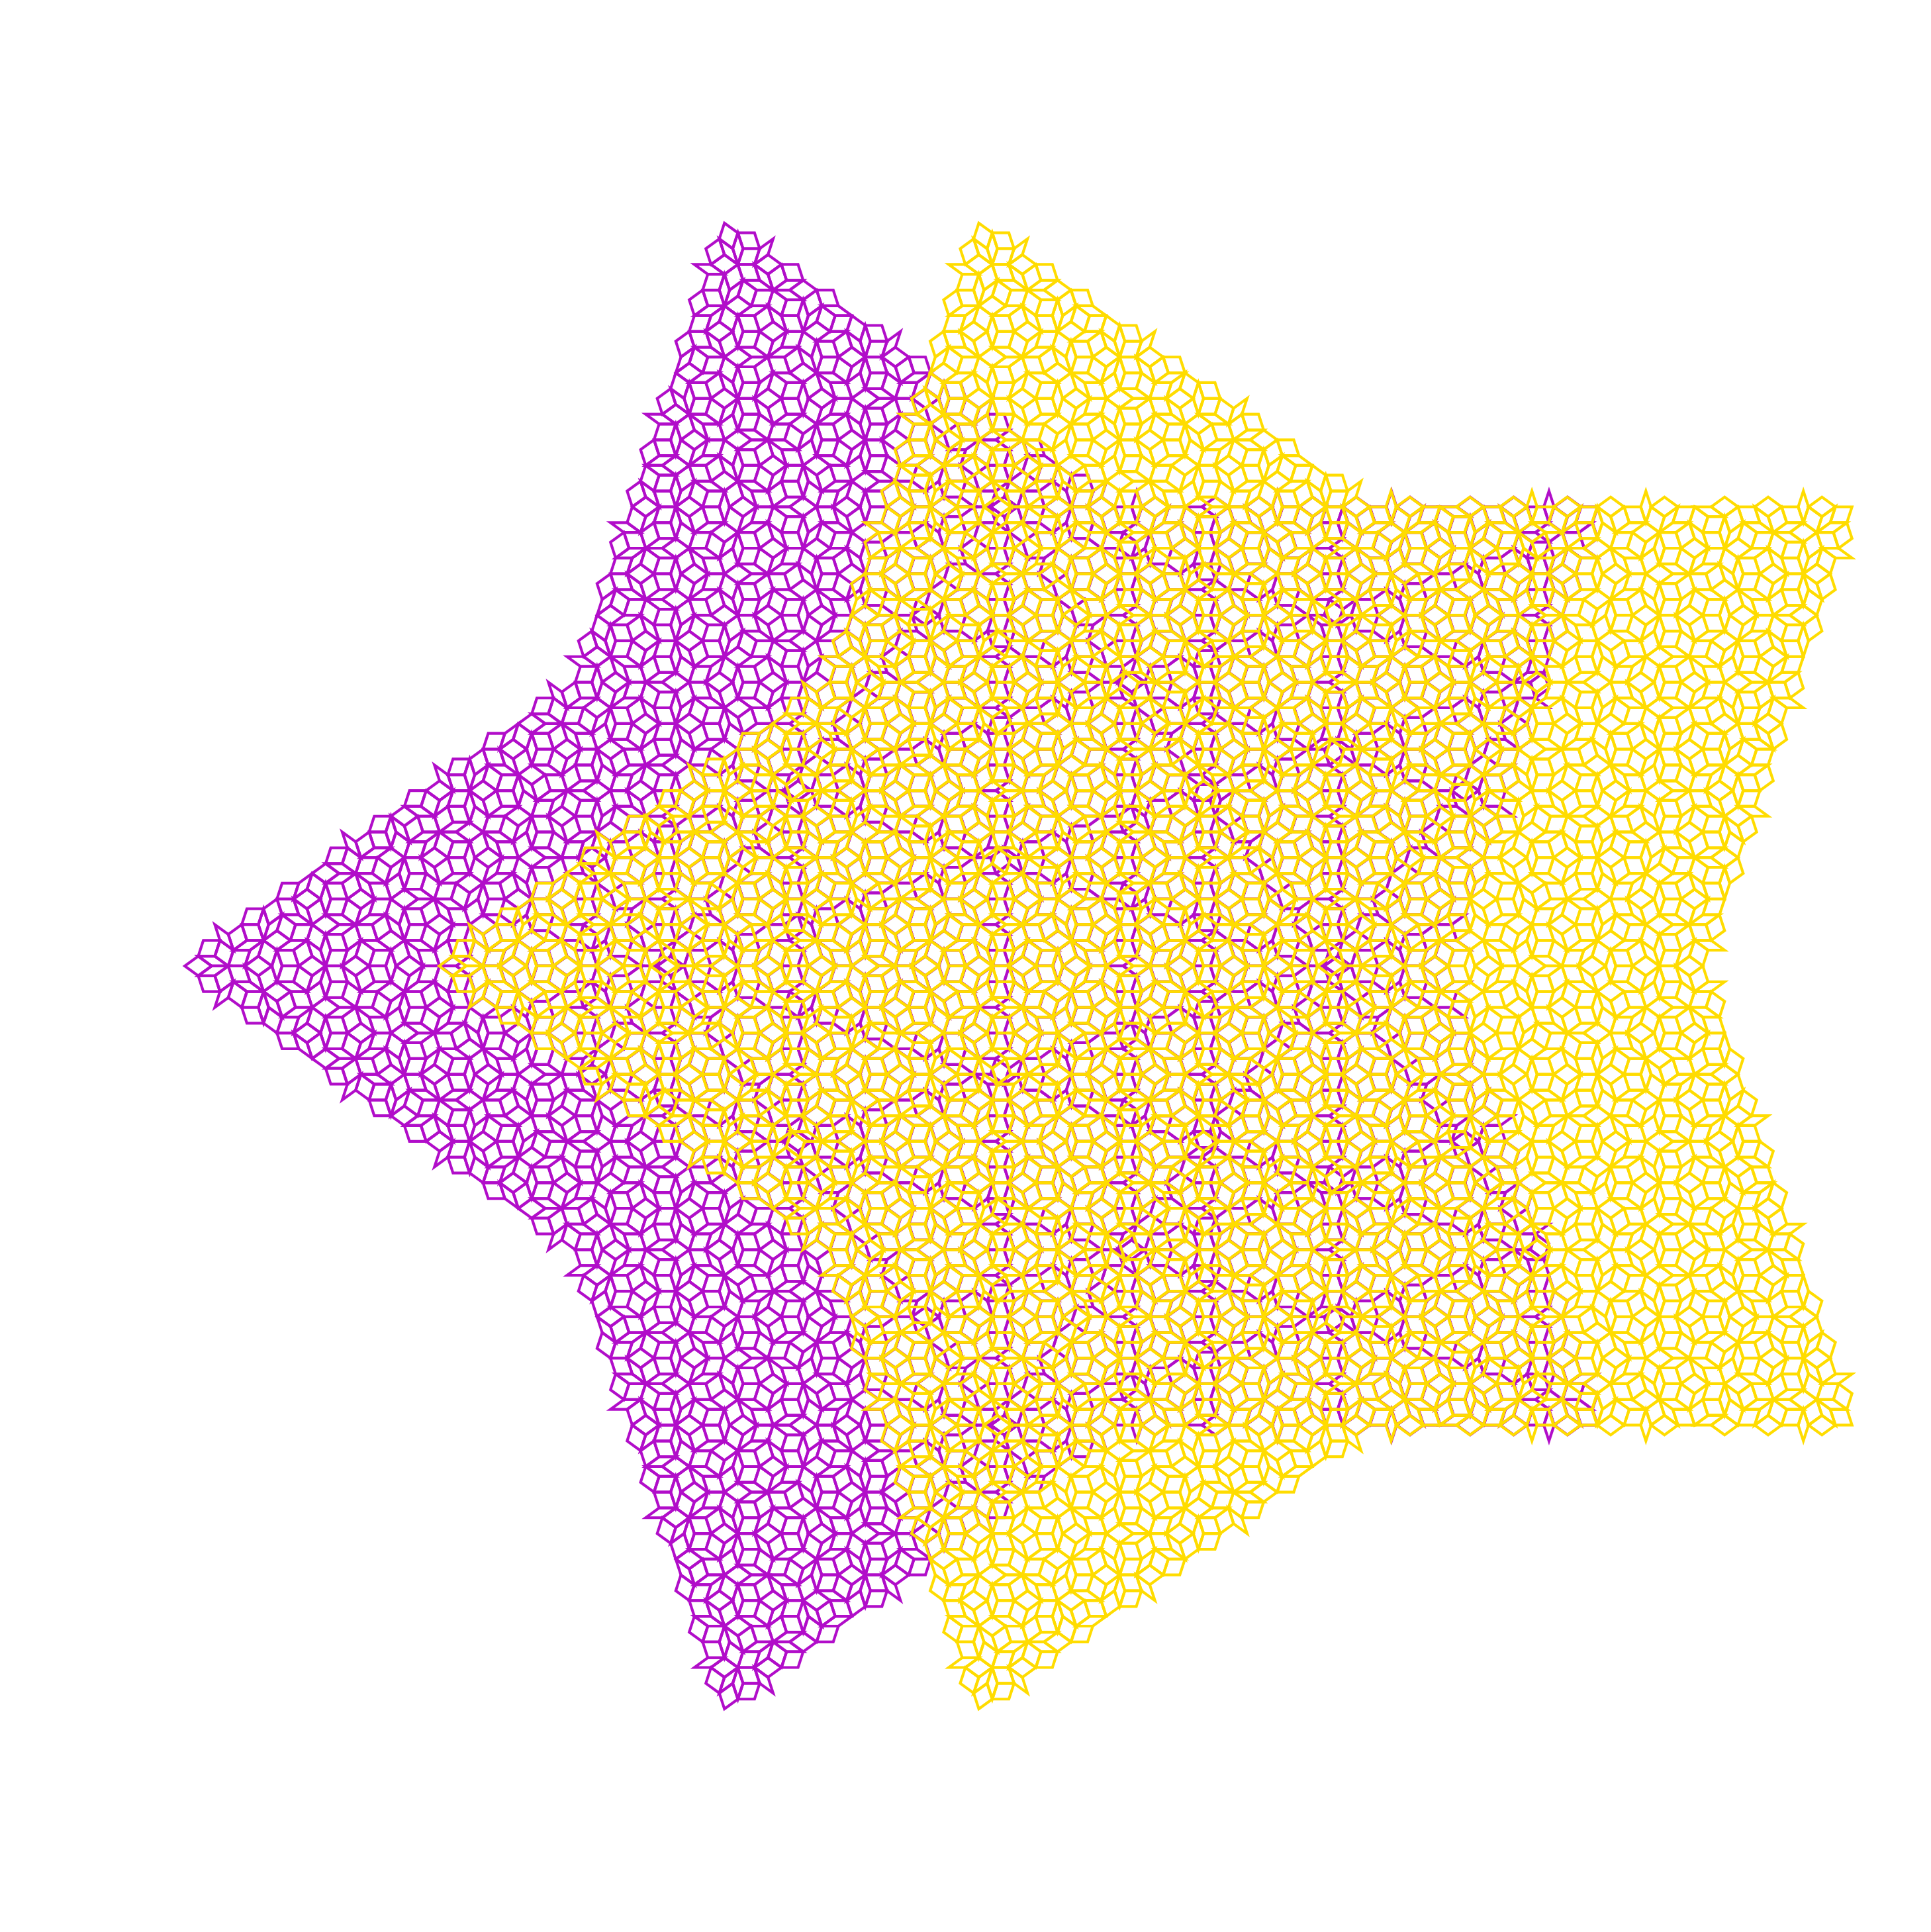
\includegraphics[width=\textwidth]{TranslateFar}
\caption{A star-shaped region of a Penrose tiling (Purple) with an identical copy of itself superimposed and translated (Yellow). Subregions where the purple tiling is invisible correspond to the regions where the translations identically match each other. Lines, or `worms', where the purple tiling is visible under the yellow tiling occur where the tiling and its translation mismatch. Note that worms travel in one of five directions.}
\label{fig:far}
\end{subfigure}

\begin{subfigure}{0.6\textwidth}
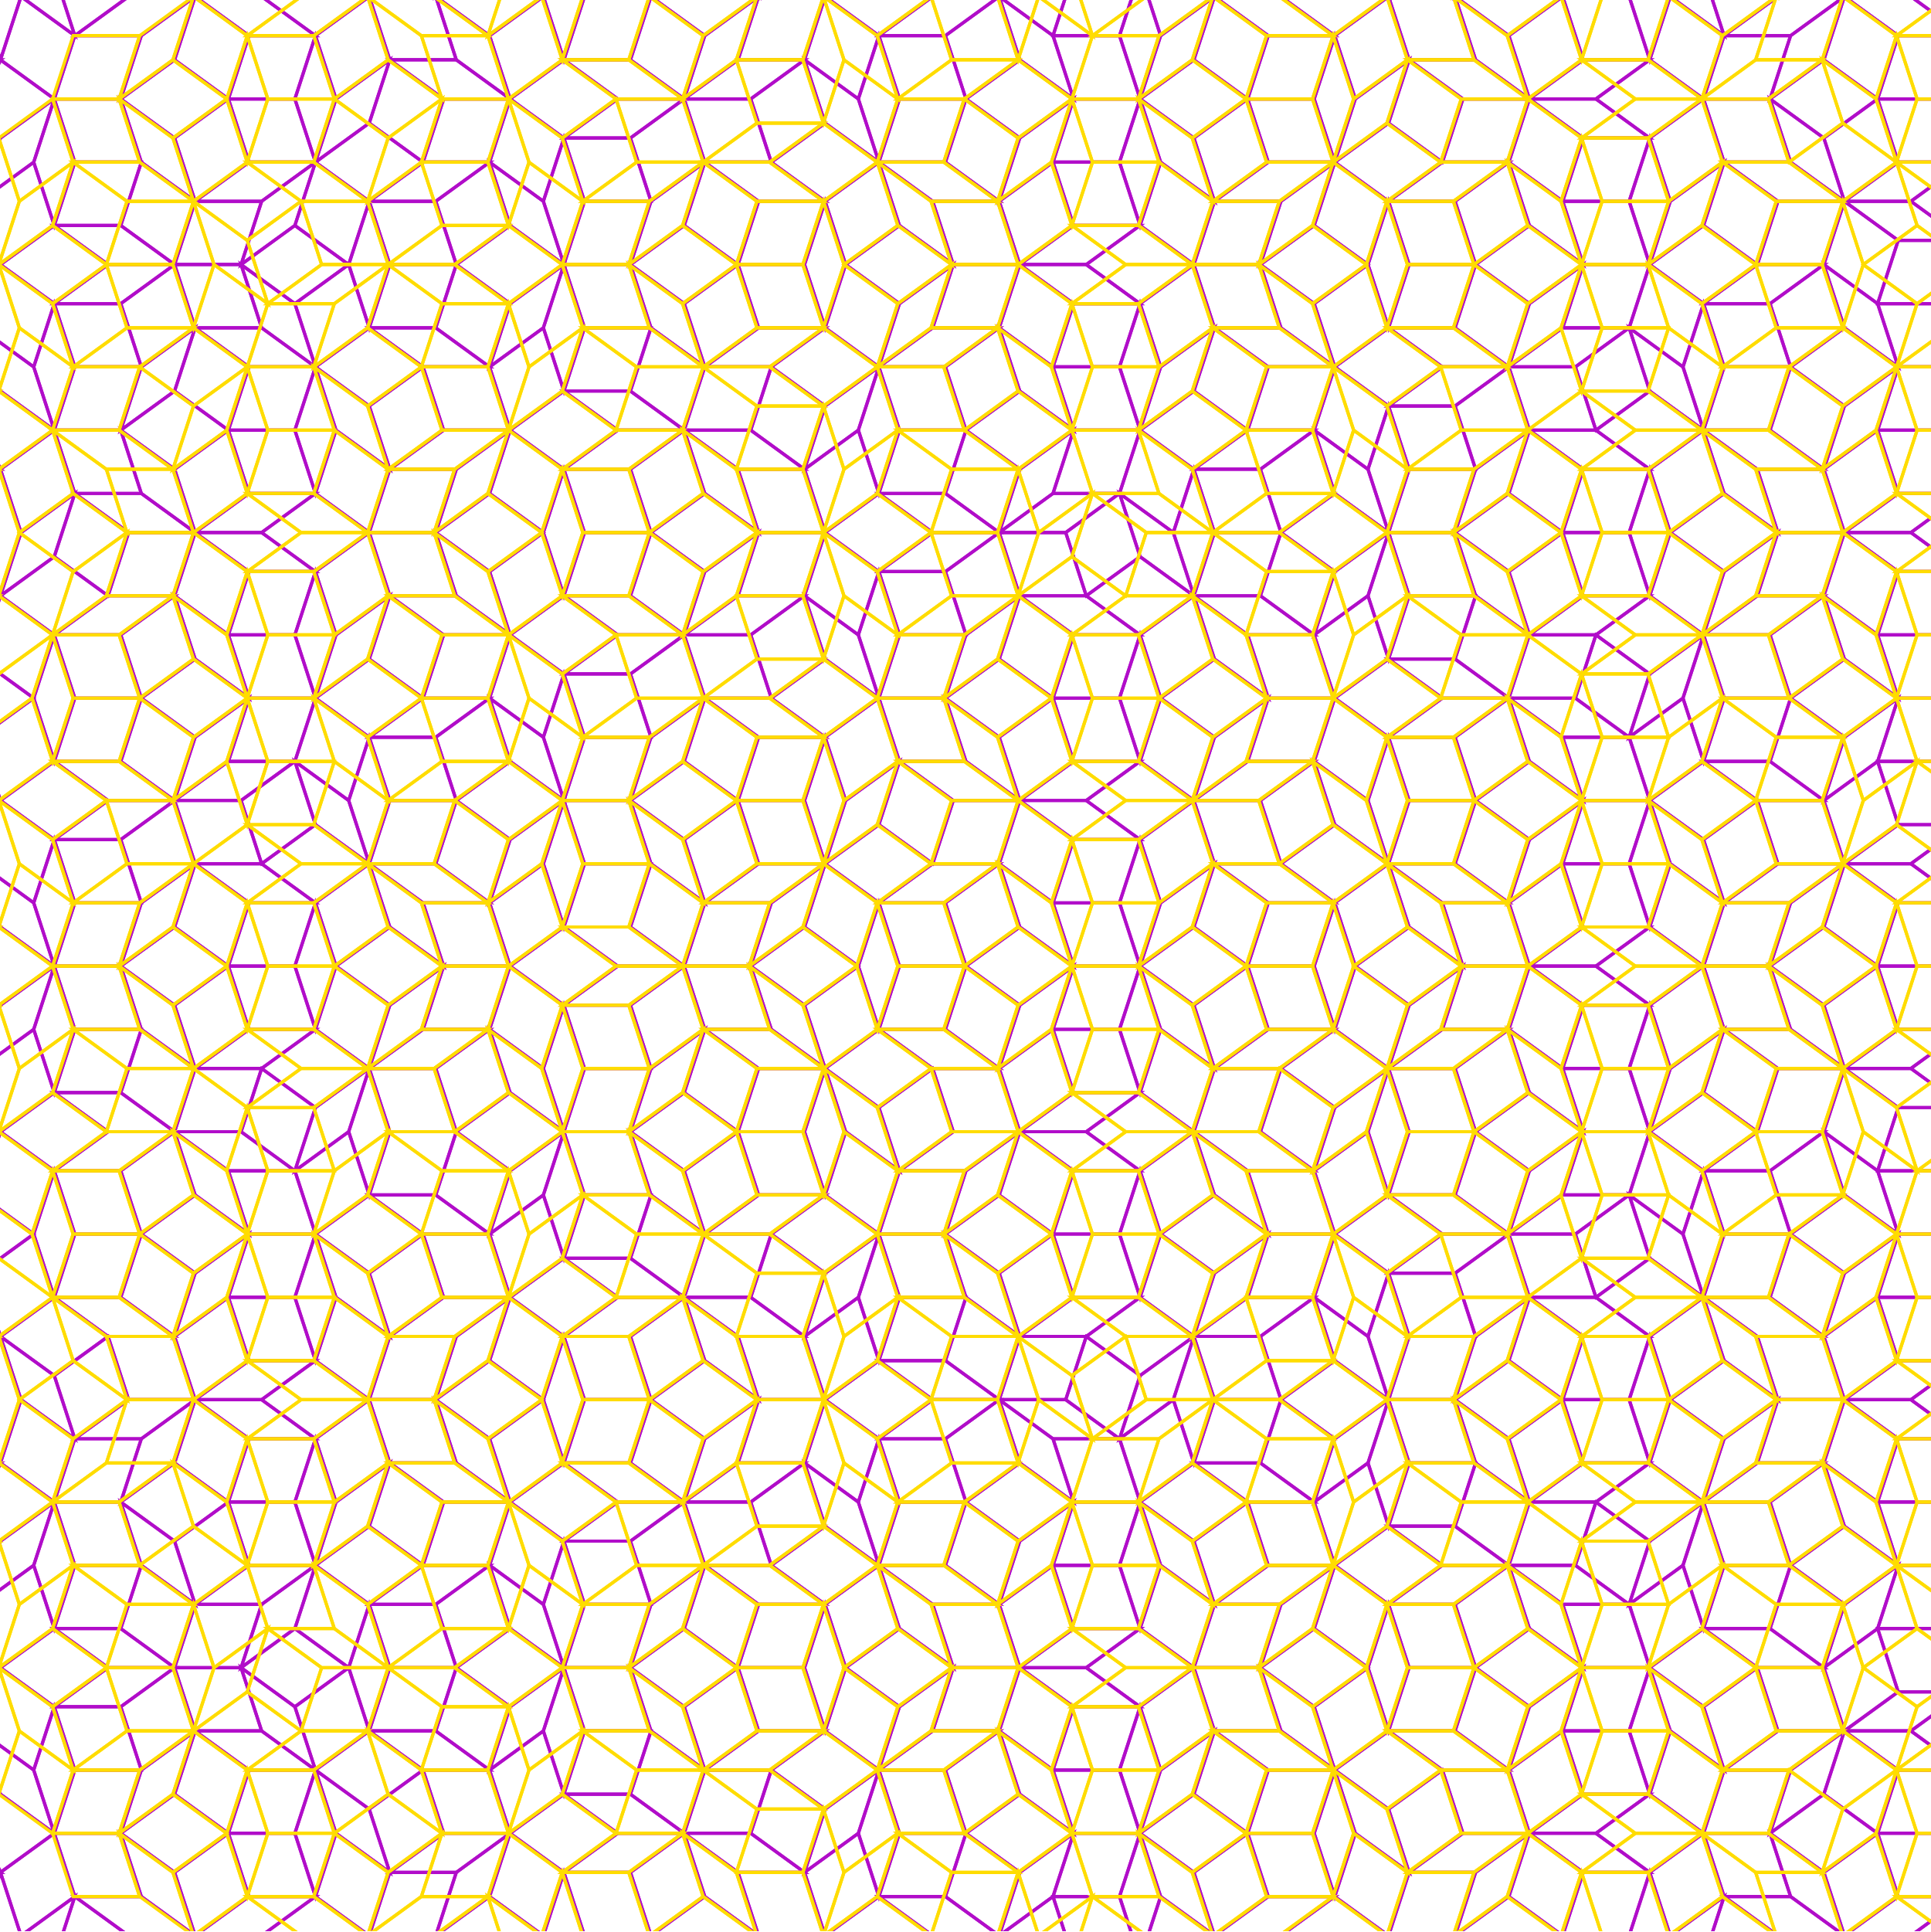
\includegraphics[width=\textwidth]{TranslateClose}
\caption{Closer view of the above overlay and translation. We can see the structure of the worms here, and how they disagree with the overlaying tiling. Notice that the worms only intersect at angles of $\frac{2\pi}{5}$}
\label{fig:close}
\end{subfigure}
\caption{Superimposed and translated Penrose tiling illustrating mismatching of patterns along worms.}
\label{fig:translations}
\end{figure}

We can see an examples of a finite worms in Fig.\ref{fig:worm}. Worms can be oriented either upwards or downwards. The mismatching which occurred in Fig.\ref{fig:translations} is the result of upwards oriented worms overlapping downwards oriented worms. 

Worms are composed of either sequences of long and short segments, where the long segment is $\phi$ times as long as the short segment.

\begin{figure}[h]
\centering
\begin{subfigure}{\textwidth}
\centering
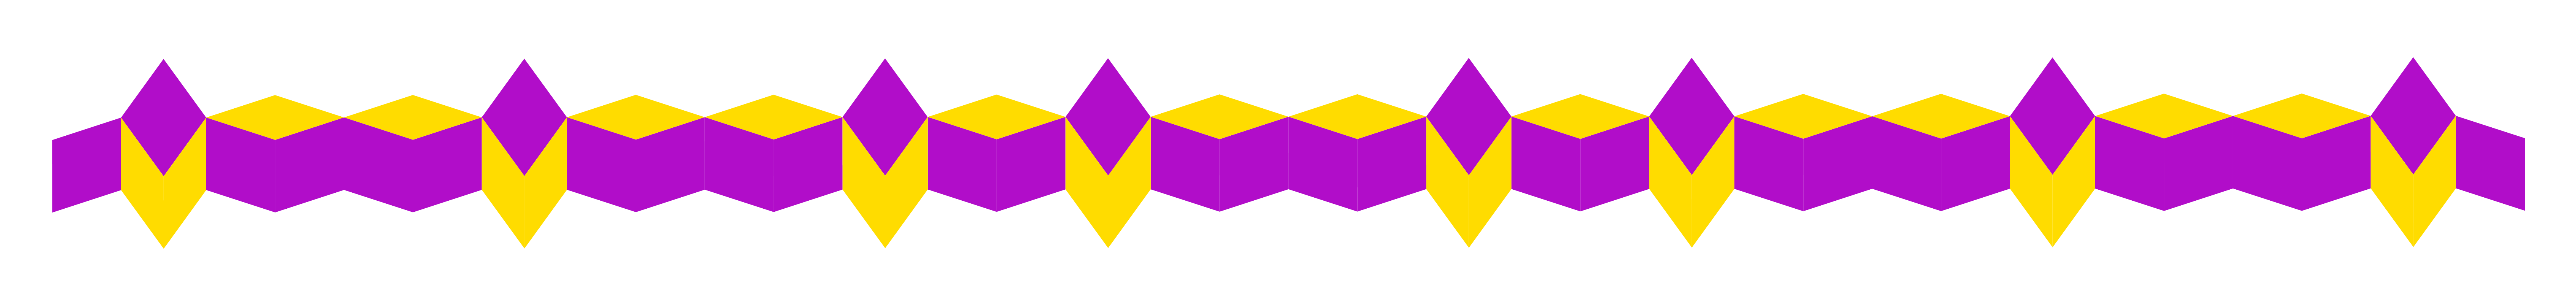
\includegraphics[width=\textwidth]{Worm}
\caption{Upwards oriented worm}
\end{subfigure}

\begin{subfigure}{\textwidth}
\centering
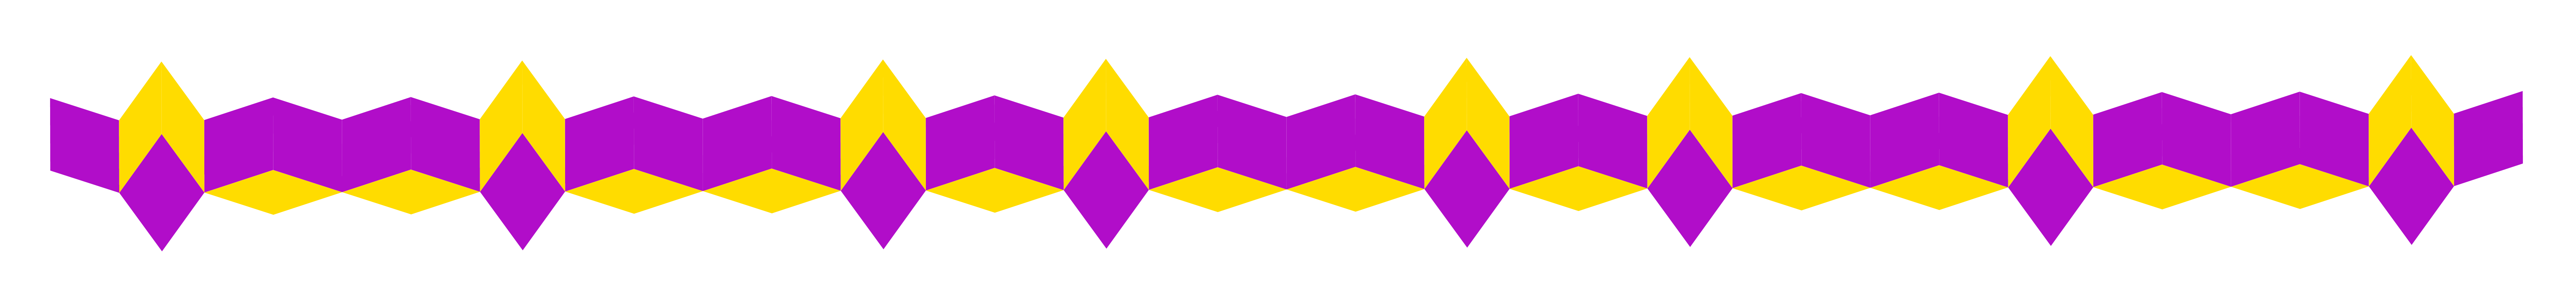
\includegraphics[width=\textwidth]{WormDown}
\caption{Downwards oriented worm}
\end{subfigure}

\caption{Oriented Worms}
\label{fig:worm}
\end{figure}

\begin{figure}[h]
\centering
\begin{subfigure}[b]{0.4\textwidth}
\centering
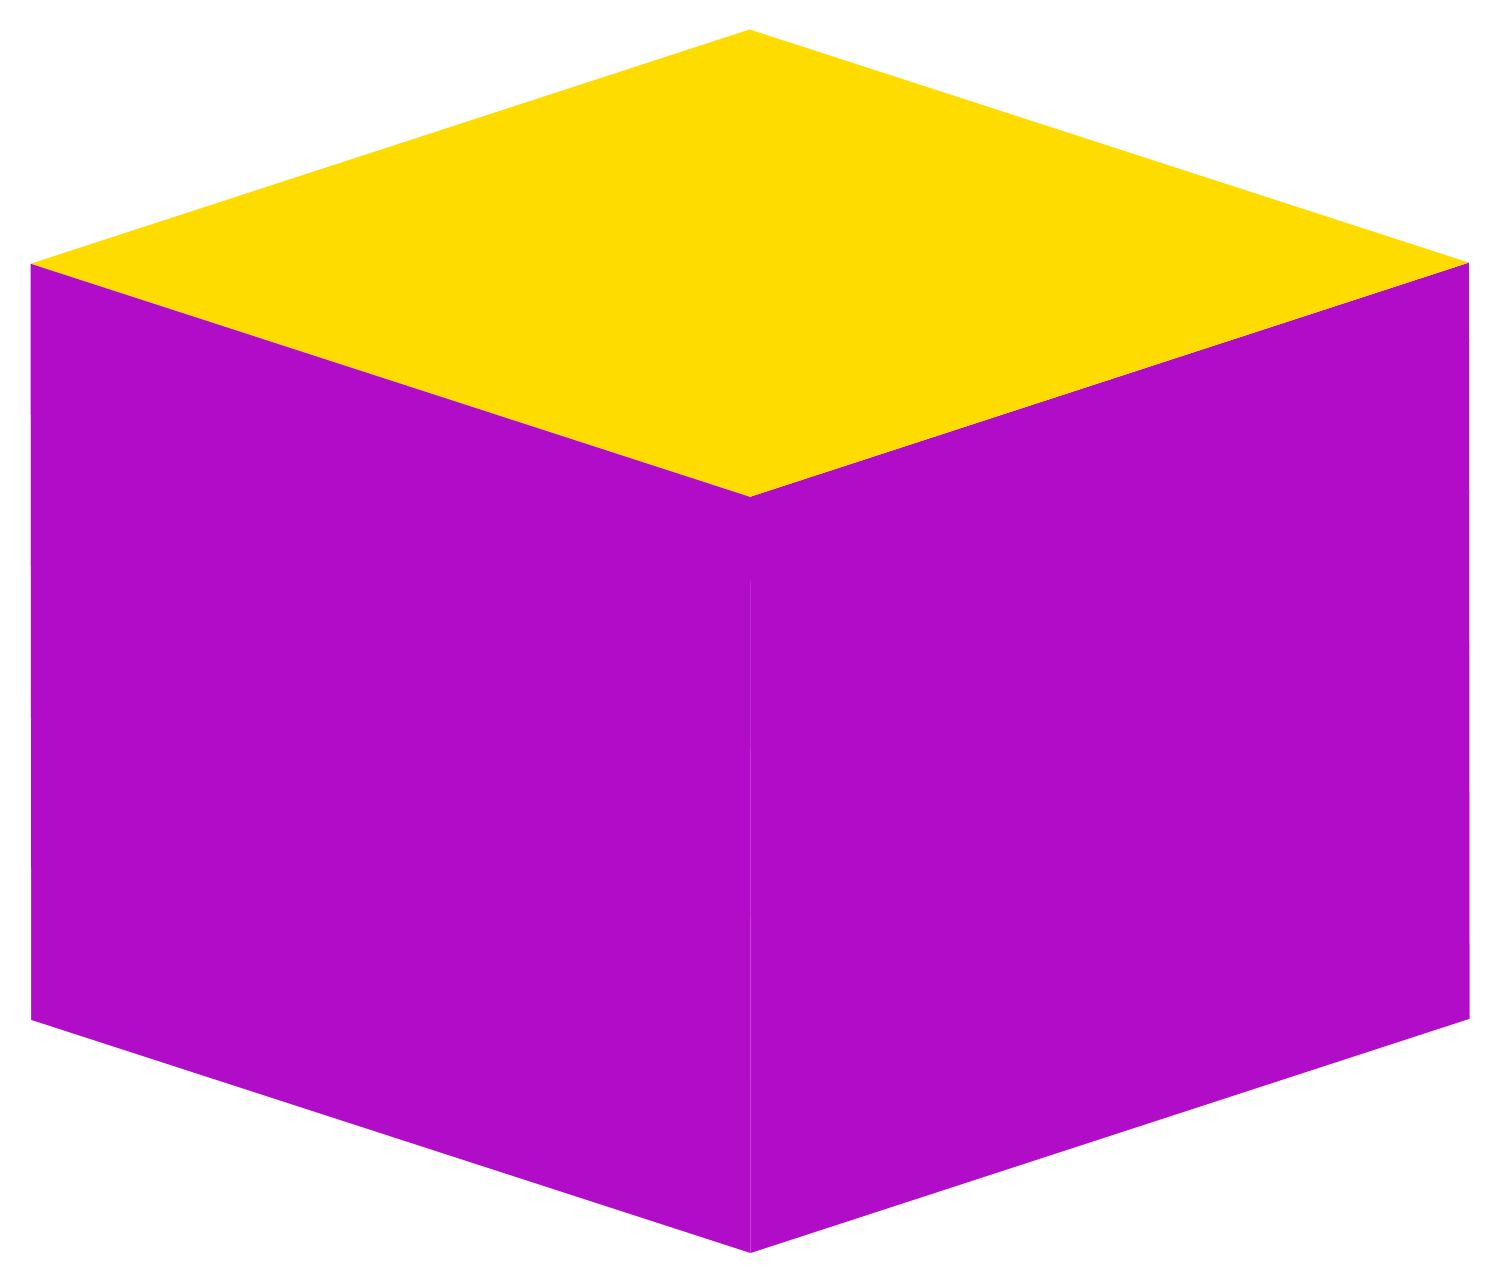
\includegraphics[width=0.7\textwidth]{WideWorm}
\caption{Long segment}
\end{subfigure}\hfill
\begin{subfigure}[b]{0.4\textwidth}
\centering

\includegraphics[width=0.4\textwidth]{TallWorm}
\caption{Short segment}
\end{subfigure}
\caption{Worm segments}
\label{fig:wormparts}
\end{figure}

As discussed previously, the Penrose tiling is non-locally constructed. That is, placement of tiles must agree with global placement conditions. As we've seen with the Up-Down method, these global conditions are determined by hierarchies of how tilings compose larger parent tiles. Worms are very apparent communicators of this global agreement information. The placement of tiles continuing the worms in either direction must correspond to valid compositions of hierarchical parent tiles. For an example of how worms can communicate non-local mistakes, see Fig.\ref{fig:wormmistakes}. For detailed descriptions of how worms communicate mistakes over arbitrarily large distances, see David Austin's AMS Feature Column \textit{Penrose Tiles Talk Across Miles} \cite{Austin2007} or Elissa Ross's Master's thesis \textit{Non-Local Growth of Penrose Tilings} \cite{Ross}.

\begin{figure}[h]
\centering
\begin{subfigure}{\textwidth}
\centering
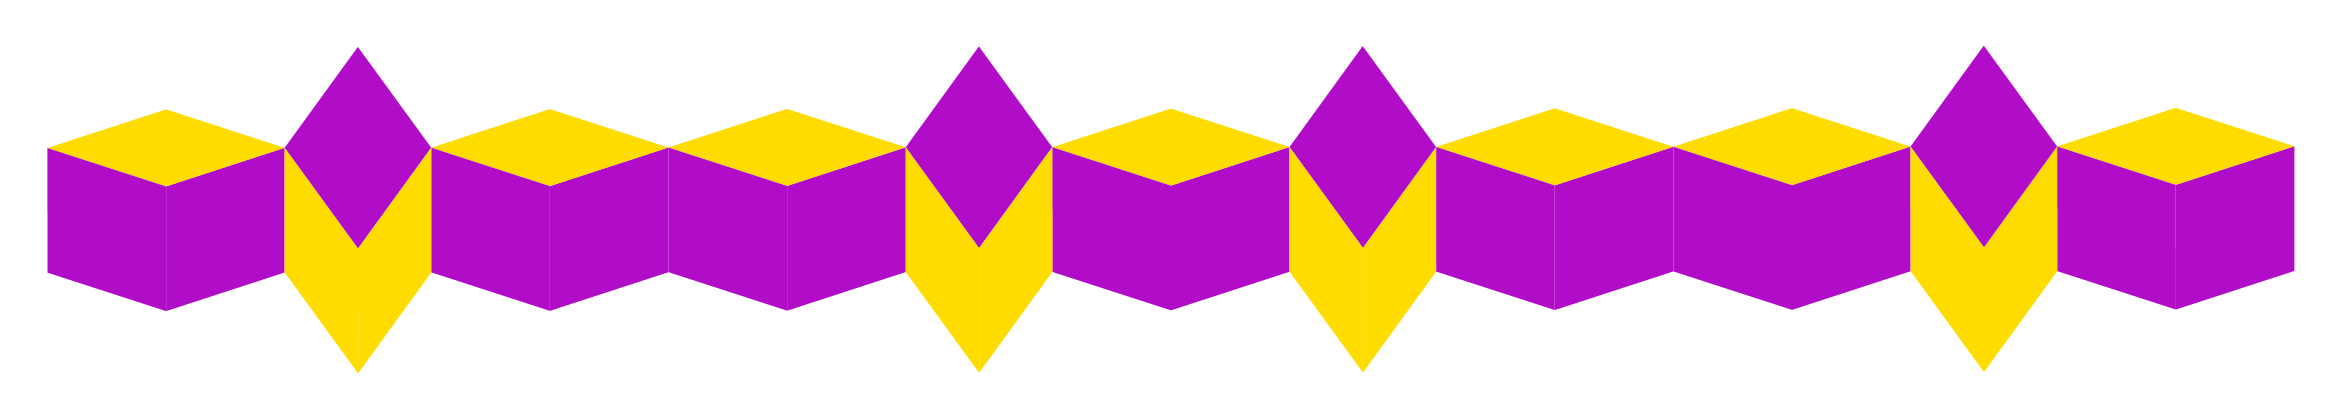
\includegraphics[width=\textwidth]{ValidWorm0}
\caption{Upwards oriented worm}
\end{subfigure}

\begin{subfigure}{\textwidth}
\centering
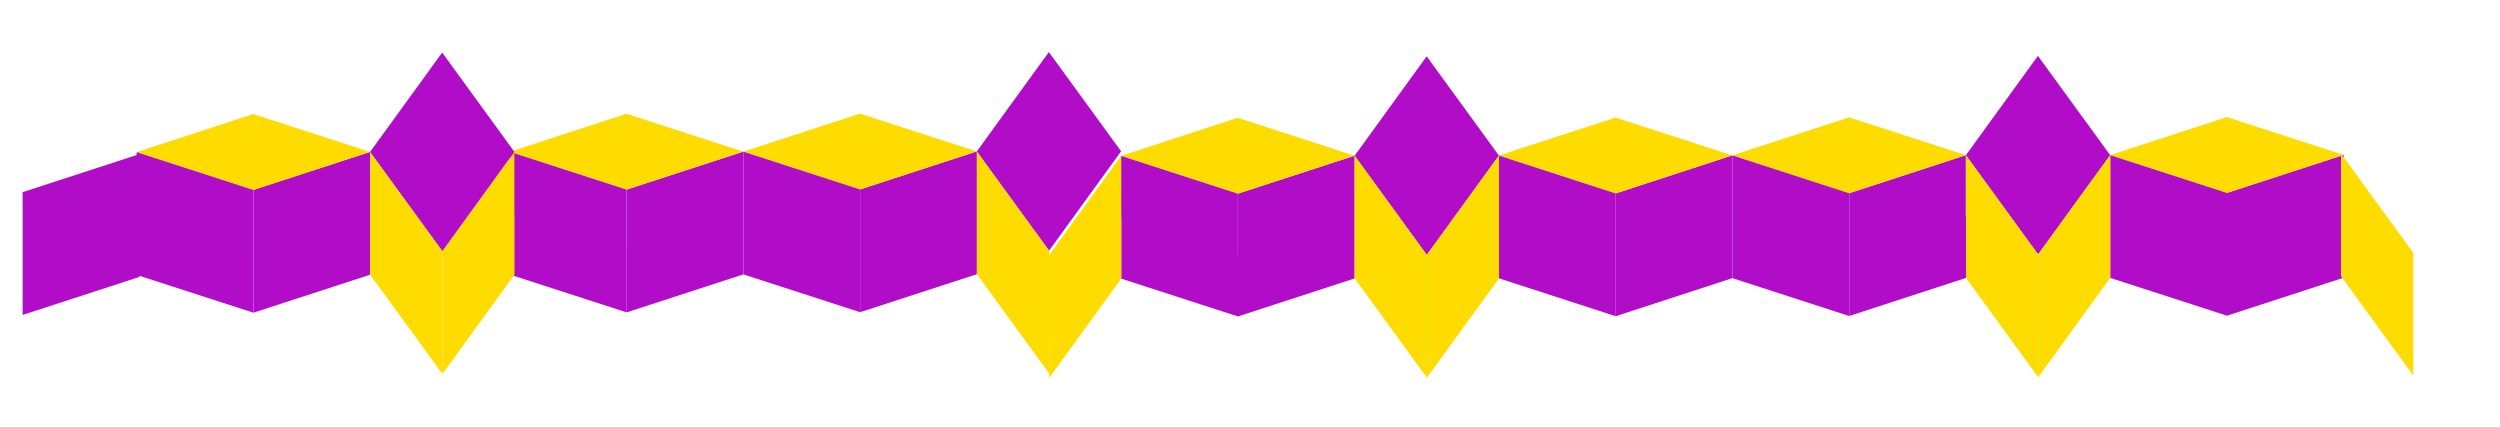
\includegraphics[width=\textwidth]{ValidWorm1}
\caption{Valid continuation of an upwards oriented worm}
\end{subfigure}

\begin{subfigure}{\textwidth}
\centering
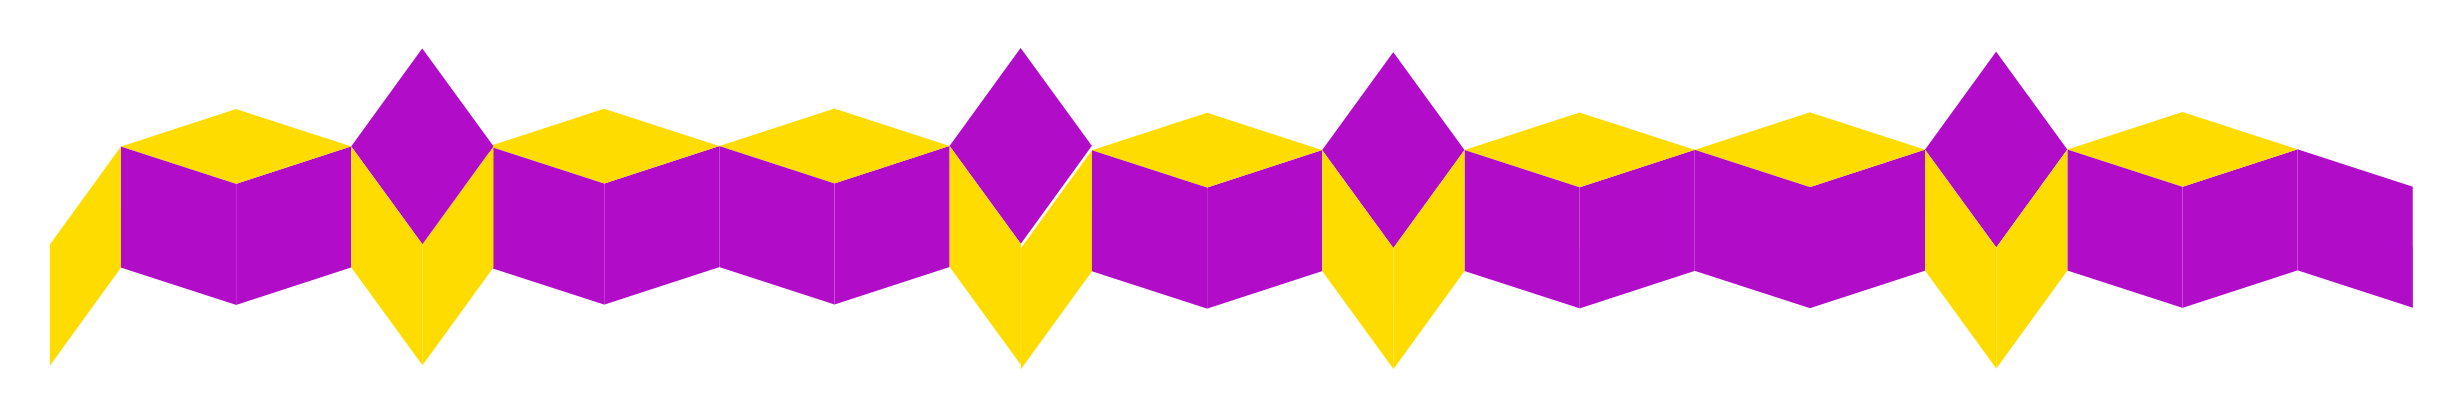
\includegraphics[width=\textwidth]{ValidWorm2}
\caption{Valid continuation of an upwards oriented worm}
\end{subfigure}

\begin{subfigure}{\textwidth}
\centering
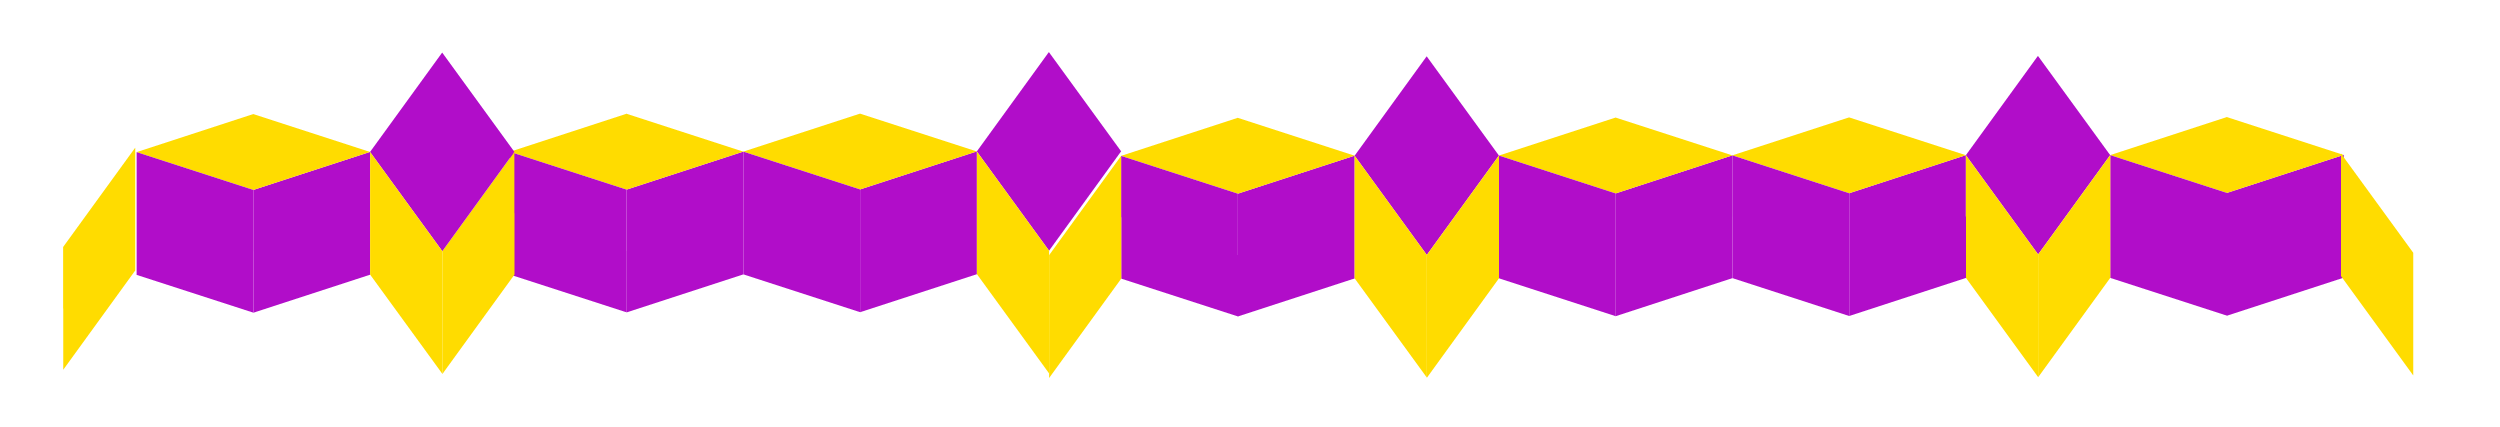
\includegraphics[width=\textwidth]{InvalidWorm}
\caption{Invalid continuation of an upwards oriented worm. This generates a mistake.}
\end{subfigure}

\begin{subfigure}{\textwidth}
\centering
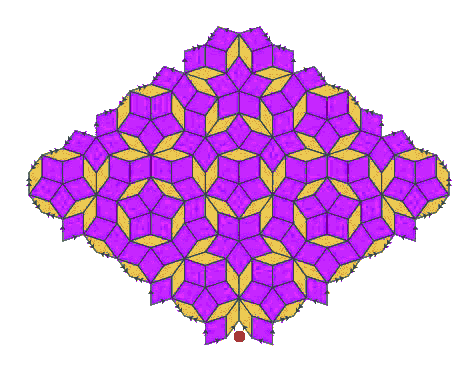
\includegraphics[width=0.5\textwidth]{illegal}
\caption{Worm mistake manifests an unfillable gap error at the red dot at the bottom of this subregion. Figure recolored from \cite{Austin2007}.}
\end{subfigure}

\caption{Continuing worms can non-locally communicate mistakes over arbitrarily large distances.}
\label{fig:wormmistakes}
\end{figure}

\end{document}